\chapter{硅基混合集成III-V波导}
\section{量子阱结构的设计}
本论文的硅基混合集成III-V光调制器是基于多量子阱(Multiple Quantum Well, MQW)的电吸收效应,这个效应也被成为量子束缚Stark(Quantum Confined Stark Effect, QCSE)现象。而对于块状材料,电吸收效应被称作Franz-Keldysh效应\cite{keldysh1958effect,franz1958einfluss}。Franz-Keldysh效应是指在外界电场的作用下,材料的能带发生倾斜,吸收峰往长波漂移,即能量低于导带和价带间隔的光子依旧能使电子从价带激发到导带。在激发的过程中,也需要考虑导带的空穴和价带的电子之间的库仑相互左右,而形成的激子。由于激子效应,吸收谱的末端处有强烈的吸收峰。对于块材料,激子效应只在没有偏压下才会明显。而在有偏压的情况下,电子和空穴受到外界电场的左右,互相分离,导致激子无法形成。对于量子结构,电子和空穴都被约束在有势垒的量子阱中。即使在外界电场的作用下,能带发生倾斜,电子和空穴在量子阱中的寿命仍然很长,依旧可以在吸收谱上观测到激子效应。另外由于量子阱中势垒的作用,电子和空穴都在分立的能级。而外界电场引起量子阱能带的倾斜,使电子和空穴分立能级的间隔缩小,从而使吸收峰快速往长波漂移。在量子阱中,这种在外界电压下,吸收峰快速往长波漂移,并且保持激子吸收的现象称之为量子束缚Stark(Quantum Confined Stark Effect, QCSE)现象\cite{miller1984band,miller1985electric}。因此,基于QCSE的电吸收光调制器具有驱动电压小,小尺寸的特点。

\begin{figure}[htb]
	\centering
	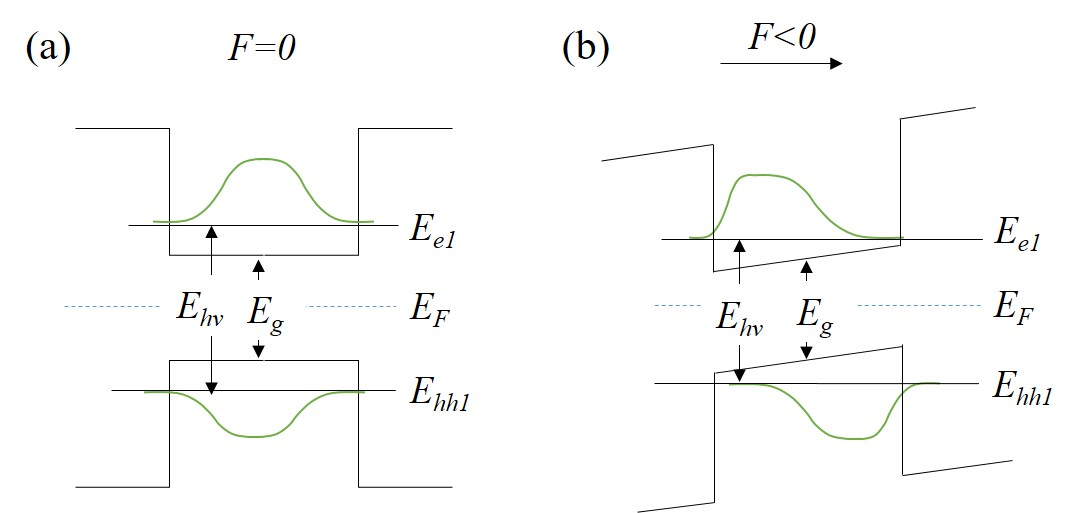
\includegraphics[width=12cm]{./Pictures/fig_ch2_band_lineup.jpg}
	\caption{ 量子阱的能带和波函数的示意图(a)有外界加电场下;(b)在外界电场的时候}
	\label{fig_ch2_band_lineup}
\end{figure}

图\ref{fig_ch2_band_lineup}(a)展示了没有外界偏压下量子阱的导带和价带,电子和空穴的波函数在空间上相互重叠,此时激子效应强度最大。当在外界电场的相互作用下,可以看到电子和空穴的分立能级的间隔变小,并且两者的波函数在空间上相错,此时激子效应的强度减弱。图\ref{fig_ch2_absorption_spec}(a,b)展示了实验测的不同偏振下量子阱的吸收谱随着外界电场的变化而变化\cite{chao1993momentum}。从中我们可以看出,外界电场使吸收谱往红移动,然后吸收谱边缘的激子吸收峰逐渐减弱,并且不同偏振下的吸收谱不同。图\ref{fig_ch2_absorption_spec}(c,d)展示了根据实验数据,里面计算得到的结果\cite{chao1993momentum}。可以看到理论和实验吻合的很好。关于量子阱中QCSE现象自从1984年在半导体量子阱材料被发现以来调\cite{miller1984band, wood1984high},依旧构建了多套完整的物理模型\cite{chuang1995physics}。下面,我们将介绍本论文采用的物理模型和计算方法。
\begin{figure}[htb]
	\centering
	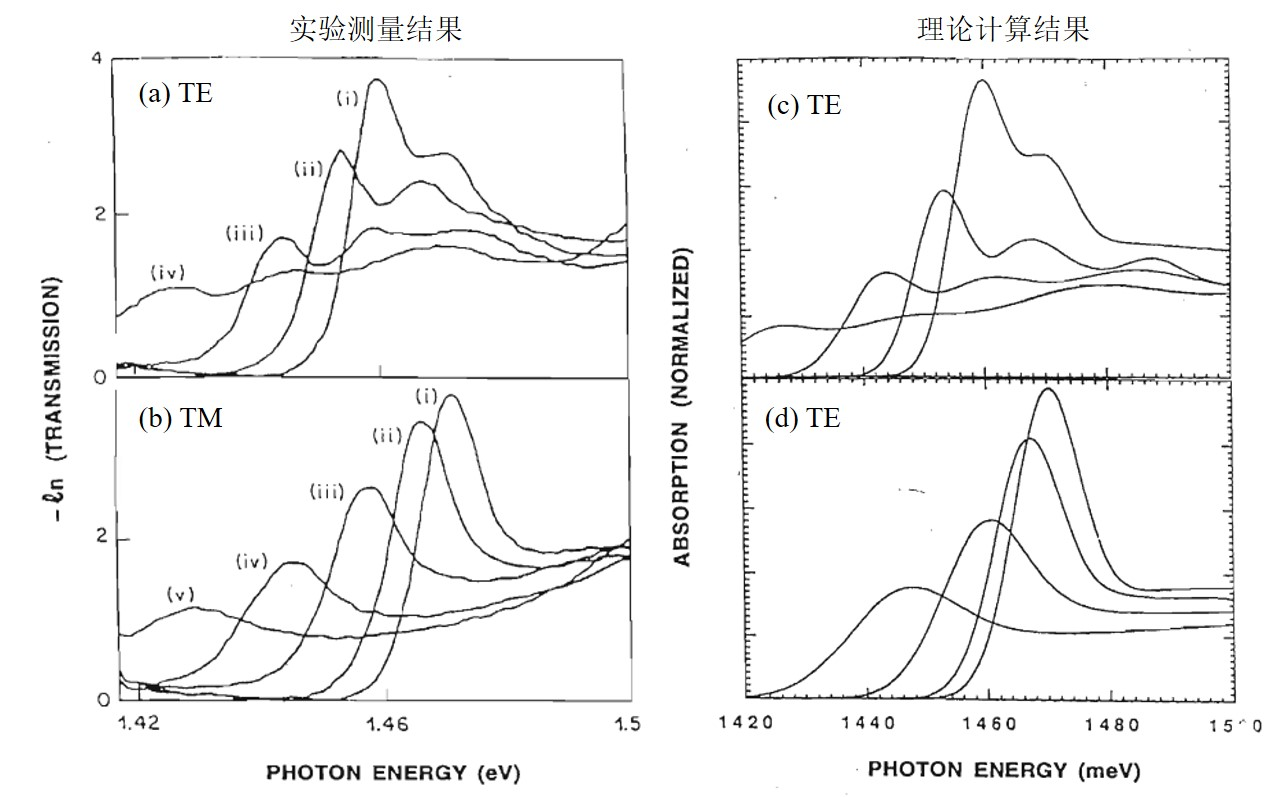
\includegraphics[width=12cm]{./Pictures/fig_ch2_absorption_spec.jpg}
	\caption{ (a,b) 实验测量的量子阱TE和TM偏振光的吸收谱\cite{chao1993momentum};(c,d) 理论计算的量子阱TE和TM偏振光的吸收谱\cite{chao1993momentum}}
	\label{fig_ch2_absorption_spec}
\end{figure}

\subsection{基本物理和数值计算}
目前计算量子阱的吸收谱商业上的软件只有一款昂贵的Harold EAM\cite{HarolEAM}软件。在此,我们采用文献[\citenum{chuang1995physics, mares1993modeling, roy1993modified, chuang1991exciton}]的方法,计算外界电场下的量子阱的吸收谱。计算吸收谱需要采用四个步骤,如图\ref{fig_ch2_flow_chart}(a)所示。通过第一步和第二布求解电子,空穴在外界下电场下的薛定谔方程\ref{Equ:Schro}得到本征能量$E$和波函数$\psi(z)$,如图\ref{fig_ch2_flow_chart}(b)所示。通过第三步和第四步求解出包含激子效应量子阱的吸收谱。
\begin{figure}[htb]
	\centering
	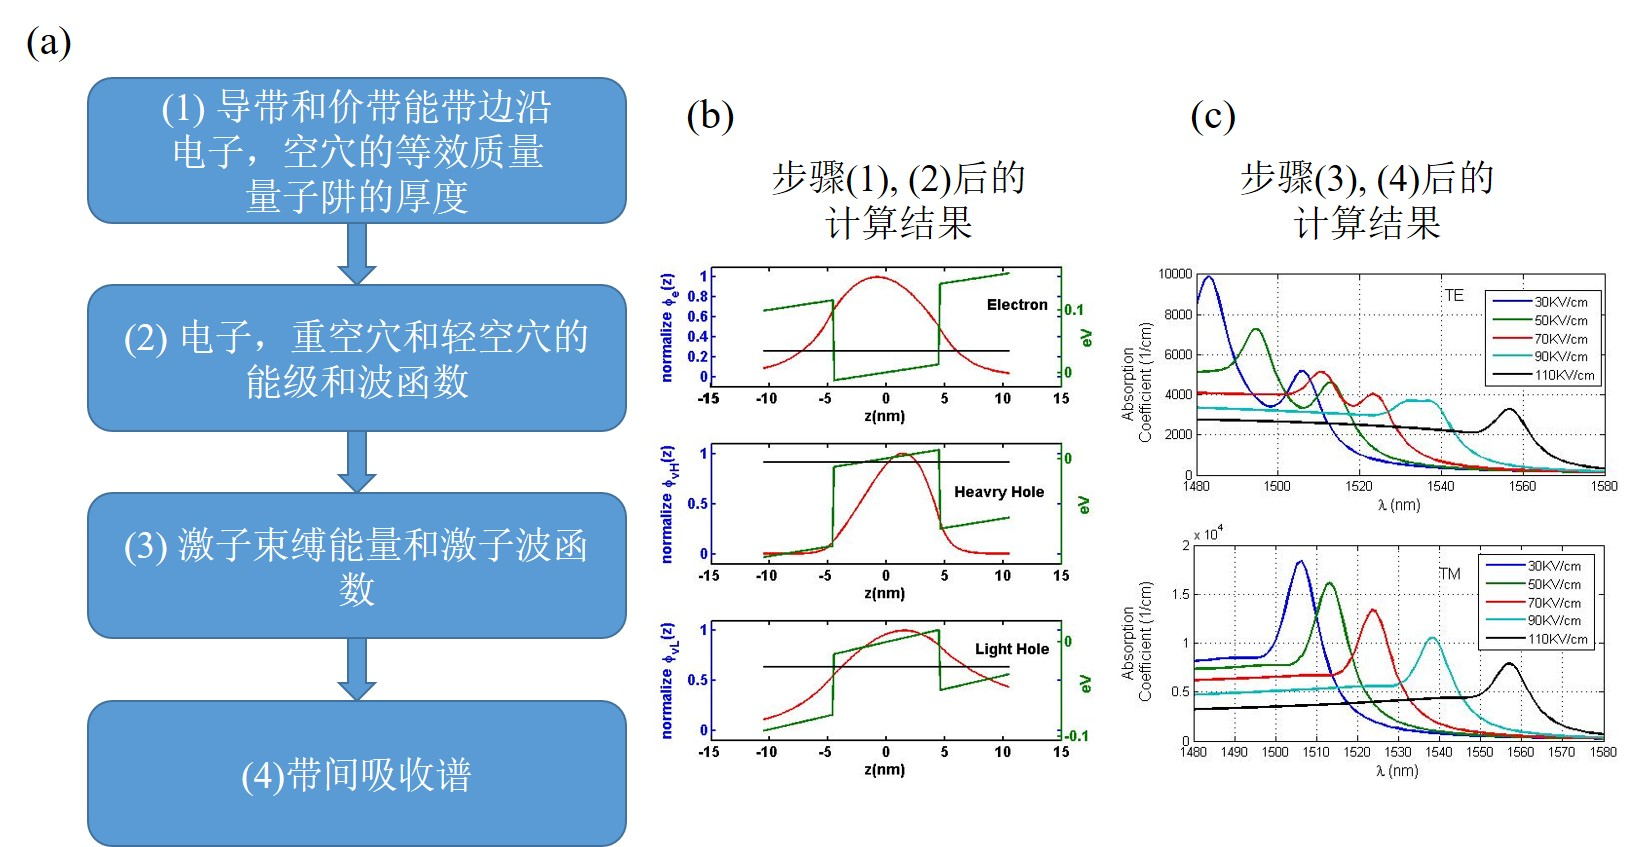
\includegraphics[width=12cm]{./Pictures/fig_ch2_flow_chart.jpg}
	\caption{(a)量子阱吸收谱的数值计算步骤;(b)第一和第二步的计算得到的电子,重空穴和轻空穴的能量和波函数;(c)第三和第四步计算得到的TE和TM偏振光的吸收谱}
	\label{fig_ch2_flow_chart}
\end{figure}

\begin{equation}
\label{Equ:Schro}
(\frac{\hbar^2}{2m}\Delta^2+V(z)+eFz)\psi(z)=E\psi(z)
\end{equation}
第一步计算材料的导带和价带的边沿结构。量子阱是由两种材料间隔排列而成。图\ref{fig_ch2_band_diagram}展示了在材料应力情况下量子阱能带边沿结构的变化\cite{chuang1995physics}。

\begin{figure}[htb]
	\centering
	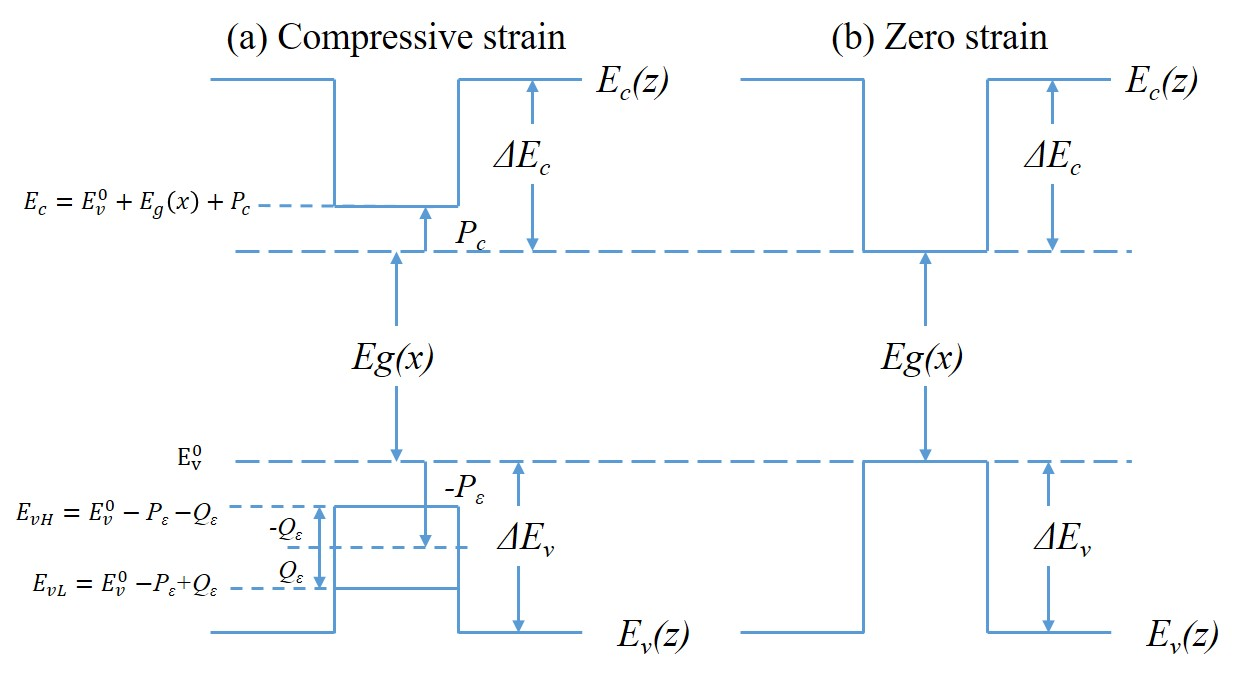
\includegraphics[width=12cm]{./Pictures/fig_ch2_band_diagram.jpg}
	\caption{有应力量子阱中的能带边沿图,(a)压缩应变;(b)张力应变}
	\label{fig_ch2_band_diagram}
\end{figure}

假设势阱中材料的晶格常熟为$a$,它在衬底晶格常数为$a_{0}$的材料上生长。那么我们可以用三个方向的应力来表式:
\begin{equation}
\label{Equ:exx}
\epsilon_{xx} = \epsilon_{yy} = \frac{a_{0}-a}{a}
\end{equation}
\begin{equation}
\label{Equ:ezz}
\epsilon_{zz} = -2\frac{C_{12}}{C_{11}}\epsilon_{xx}
\end{equation}
其中$C_{11}$和$C_{12}$是材料的弹性刚性常数(Elastic Stiffness Constants)。当$\epsilon_{zz}>0$时,材料处于压缩应变(Compressive Strain);当$\epsilon_{zz}>0$时,材料处于拉伸应变(Tensile Strain)。图\ref{fig_ch2_band_diagram}(a,b)展示了量子阱在有压缩应变和无应变情况下的能带的变化。通过比较,我们可以看到,导带上能带边沿$E_c$在受到压缩应变时,移动了$P_{c}$。表达式如下:
\begin{equation}
\label{Equ:Pc}
P_{c} = a_{c}(\epsilon_{xx}+\epsilon_{yy}+\epsilon_{zz})
\end{equation}
\begin{equation}
\label{Equ:Econ}
E_{c} = E_{v}^{0}(x)+E_{g}(x)+P_{c}
\end{equation}
其中$a_{c}$是导带的变形势能(Deformation Potentials),$E_v^0(x)$是材料在没有应变时导带的边沿,$E_{g}(x)$是材料没有应变时的导带和价带间隔,他们需要通过实验测试或者依旧材料的基本组分x查表拟合获得\cite{chuang1995physics,li2000material}。

在价带上,收到应变的影响,空穴分裂成重空穴和轻空穴,能带边沿分别是$E_{vH}$和$E_{vL}$。它们能带边沿的均值移动量是$P_{\epsilon}$,裂量是$Q_{\epsilon}$。具体表达式如下:
\begin{equation}
\label{Equ:Pe}
P_{\epsilon} = -a_{v}(\epsilon_{xx}+\epsilon_{yy}+\epsilon_{zz})
\end{equation}
\begin{equation}
\label{Equ:Qe}
Q_{\epsilon} = -\frac{b}{2}(\epsilon_{xx}+\epsilon_{yy}-2\epsilon_{zz})
\end{equation}
\begin{equation}
\label{Equ:EvH}
E_{vH} = E_{v}^{0}(x)-P_{\epsilon}-Q_{\epsilon}
\end{equation}
\begin{equation}
\label{Equ:EvL}
E_{vL} = E_{v}^{0}(x)-P_{\epsilon}+Q_{\epsilon}
\end{equation}
其中$a_{v}$和$b$是变形势能。利用公式\ref{Equ:Econ},\ref{Equ:EvH}、\ref{Equ:EvL}计算量子阱两种材料的能带边缘,就可以获得薛定谔方程中的电子,轻空穴和重空穴的势能$V(z)$。

在应力作用下,由于重空穴和轻空穴产的能带生劈裂,其等效质量,我们需要采用Luttinger parameters$\gamma_1, \gamma_2$计算。如下式所示:
\begin{equation}
\label{Equ:eff_mass_z}
\frac{m_{vH}^z}{m_0}=\frac{1}{\gamma_1-2\gamma_2}~~~~~~~~~~\frac{m_{vL}^z}{m_0}=\frac{1}{\gamma_1+2\gamma_2}
\end{equation}
\begin{equation}
\label{Equ:eff_mass_xy}
\frac{m_{vH}^{xy}}{m_0}=\frac{1}{\gamma_1+\gamma_2}~~~~~~~~~~\frac{m_{vL}^{xy}}{m_0}=\frac{1}{\gamma_1-\gamma_2}
\end{equation}
其中公式\ref{Equ:eff_mass_z}和公式\ref{Equ:eff_mass_xy}分别是计算垂直与量子阱方向(即z方向)和水平方向重空穴和轻空穴的等效质量\cite{eppenga1987new}。

我们用于硅基混合集成III-V电吸收光调制器的多量子阱中,单个量子阱的势阱(Well)和势垒(Barrier)分别是:In\SB{0.65}Al\SB{0.09}Ga\SB{0.26}As和In\SB{0.42}Al\SB{0.17}Ga\SB{0.39}As。从文献[\citenum{chuang1995physics,li2000material}],根据它们各个元素,再依据\ref{Equ:Econ},\ref{Equ:EvH}、\ref{Equ:EvL}、\ref{Equ:eff_mass_z}、\ref{Equ:eff_mass_xy}式可以获得如下表\ref{QWmaterial}的量子阱材料数据。其中势阱受到了0.82\%的压缩应变,势垒受到了0.73\%的拉伸应变。
{
	\begin{table}[htb]
		\zihao{5}
		\caption{量子阱材料数据。E\SB{vL}:轻空穴的能带边沿;E\SB{vH}:重空穴的能带边沿;E\SB{c}:导带的能带边沿;$m_{vL}^z$:轻空穴z向等效质量;$m_{vL}^{xy}$:轻空穴xy向等效质量;$m_{vH}^z$:重空穴z向等效质量;$m_{vH}^{xy}$:重空穴xy向等效质量;$m_e$:电子等效质量;$m_0$:电子质量。}
		\label{QWmaterial}
		\centering
		\begin{tabular}[t]{ccccccccc}
			\hline
			类型  & E\SB{vL}(eV) & E\SB{vH}(eV) & E\SB{c}(eV) & $m_{vL}^z$ ($m_0$) & $m_{vL}^{xy}$ ($m_0$) & $m_{vH}^{z}$ ($m_0$) & $m_{vH}^{xy} $ ($m_0$) & $m_e$ ($m_0$)\\
			\hline
			Well & -6.7220 & -6.6695 & -5.9031 & 0.0374 & 0.1216 & 0.4874 & 0.0486 & 0.0457\\
			Barrier& -6.7573 & -6.8114 & -5.7680 & 0.0481 & 0.1498 & 0.5080 & 0.0621 & 0.0641\\
			\hline
		\end{tabular}
	\end{table}
}

第二步数值求解公式\ref{Equ:Schro}计算电子,重空穴和轻空穴在在一维势阱中的能级和波函数。在此我们采用的是基于传输矩阵的求解方法\cite{chuang1995physics}。首先我们将势能$V(z)+eFz$均匀分解很小的区域如图\ref{fig_ch2_divide_potential}所示。
\begin{figure}[htb]
	\centering
	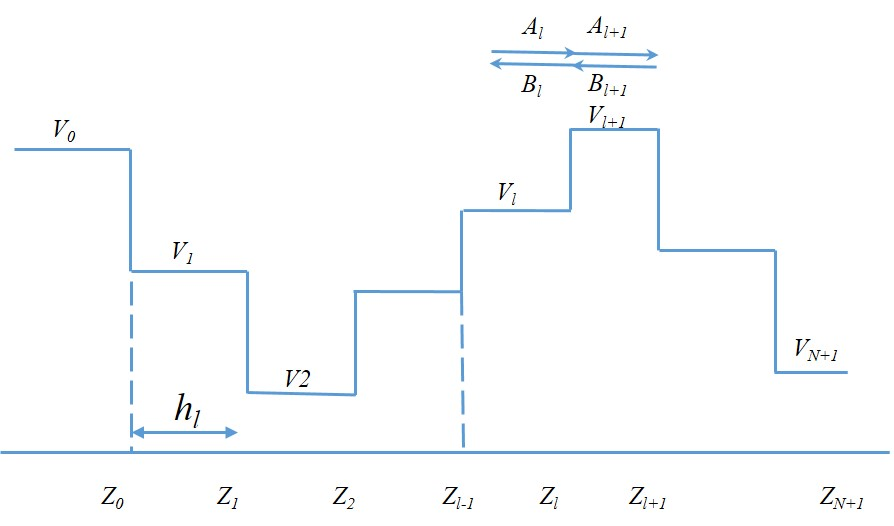
\includegraphics[width=12cm]{./Pictures/fig_ch2_divide_potential.jpg}
	\caption{将势能均匀划分成很小区域的示意图}
	\label{fig_ch2_divide_potential}
\end{figure}

假设在区域$l$,$z_{l-1} \leqslant z \leqslant z_{l}$,势能为$V_l$,粒子质量为$m_l$,那么其波函数$\psi(z)$的解为:
\begin{equation}
\label{Equ:generalsolutionsch}
\psi(z) = A_le^{ik_l(z-z_l)}+B_le^{-ik_l(z-zl)}
\end{equation}
其中区域$l$的波数$k_l$可以用本征能量$E$来表示:
\begin{equation}
\label{Equ:kl}
k_l = \sqrt{\frac{2m_l}{\hbar^2}(E-V_l)}
\end{equation}
再利用每个区域边间上$\psi(z)$和$(1/m(z))d\psi(z)/dz$连续的条件,我们可以获得区域$l+1$的系数$A_{l+1}$和$B_{l+1}$与区域$l$的系数$A_l$和$B_l$的关系:
\begin{equation}
\label{Equ:ABrelation}
\begin{bmatrix}
A_{l+1}\\
B_{l+1}
\end{bmatrix} = \textbf{F}_{(l+1)l}\begin{bmatrix}
A_{l}\\
B_{l}
\end{bmatrix}
\end{equation}
其中$\textbf{F}_{(l+1)l}$可以表示为:
\begin{equation}
\label{Equ:Fdetail}
\textbf{F}_{(l+1)l} = \frac{1}{2}\begin{bmatrix}
(1+P_{(l+1)l})e^{ik_{l+1}h_l}&(1-P_{(l+1)l})e^{ik_{l+1}h_l}\\
(1-P_{(l+1)l})e^{-ik_{l+1}h_l}&(1+P_{(l+1)l})e^{-ik_{l+1}h_l}
\end{bmatrix}
\end{equation}
其中$P_{(l+1)l}$可以表示为:
\begin{equation}
\label{Equ:Pdetail}
P_{(l+1)l} = \frac{m_lk_{l+1}}{m_{l+1}k_{l}}
\end{equation}
因此,我们可以得到第一个区域系数$A_{0}$和$B_{0}$和最后一个区域系数$A_{N+1}$和$B_{N+1}$的关系:
\begin{equation}
\label{Equ:Fmulti}
\begin{bmatrix}
A_{N+1}\\
B_{N+1}
\end{bmatrix} = \textbf{F}_{(N+1)N}\textbf{F}_{N(N-1)}\cdots\textbf{F}_{21}\textbf{F}_{10}\begin{bmatrix}
A_{0}\\
B_{0}
\end{bmatrix}
\end{equation}
由于第一区域和最后区域波函数一般要衰减的,因此$A_0 = 0$,$B_{N+1} = 0$。另外我们将矩阵的连乘写成如下形式:
\begin{equation}
\label{Equ:Fsimple}
\textbf{F}_{(N+1)N}\textbf{F}_{N(N-1)}\cdots\textbf{F}_{21}\textbf{F}_{10} = \begin{bmatrix}
f_{11}&f_{12}\\
f_{21}&f_{22}
\end{bmatrix}
\end{equation}
因此公式\cite{Equ:Fmulti}可以写成如下形式:
\begin{equation}
\label{Equ:Fmulti}
\begin{bmatrix}
A_{N+1}\\
0
\end{bmatrix} = \begin{bmatrix}
f_{11}&f_{12}\\
f_{21}&f_{22}
\end{bmatrix}
\begin{bmatrix}
0\\
B_{0}
\end{bmatrix}
\end{equation}
因此,我们获得了求解借本征量能$E$的方程:
\begin{equation}
\label{Equ:sloveE}
f_{22}(E) = 0
\end{equation}
利用牛顿迭代法或者其他数值方法我们可以获得$E$的数值。然后公式\ref{Equ:kl},\ref{Equ:Pdetail},\ref{Equ:Fdetail}反推得到$\textbf{F}$。再假设$B_{0}$的数值,利用公式\ref{Equ:Fmulti},我们就可以得到每个区域波函数$\psi(z)$。最后,根据粒子在整个空间出现的概率为1,对波函数进行归一化。图\ref{fig_ch2_bias_wavefunction}(a,b)分别展示了在没有偏压和2 KV/cm的偏压下,利用传输矩阵,计算得到的电子,重空穴,轻空穴的最低能级和对应波函数。在没有偏压下,电子和重空穴之间的能量间隔是$E_{e-vH} = 0.7997 eV$,当偏压为2 KV/cm时,其间隔变为$E_{e-vH} = 0.7979$,标明吸收峰蓝移了$\Delta E_{e-vH} = 1.8 meV$。电子和轻空穴在没有和2 KV/cm下的能量间隔$E_{e-vL}$分别是$0.8649 eV$和$0.8612 eV$,蓝移量为 $\Delta E_{e-vL} = 3.7 mV$。$\Delta E_{e-vL}$ 大于 $\Delta E_{e-vH}$是由于,如表\ref{QWmaterial}所示,轻空穴的等效质量少于重空穴,并且轻空穴的势垒和势阱的能带变差相比重空穴而言更小,因此轻空穴更容易受到势能变化的影响。
\begin{figure}[htb]
	\centering
	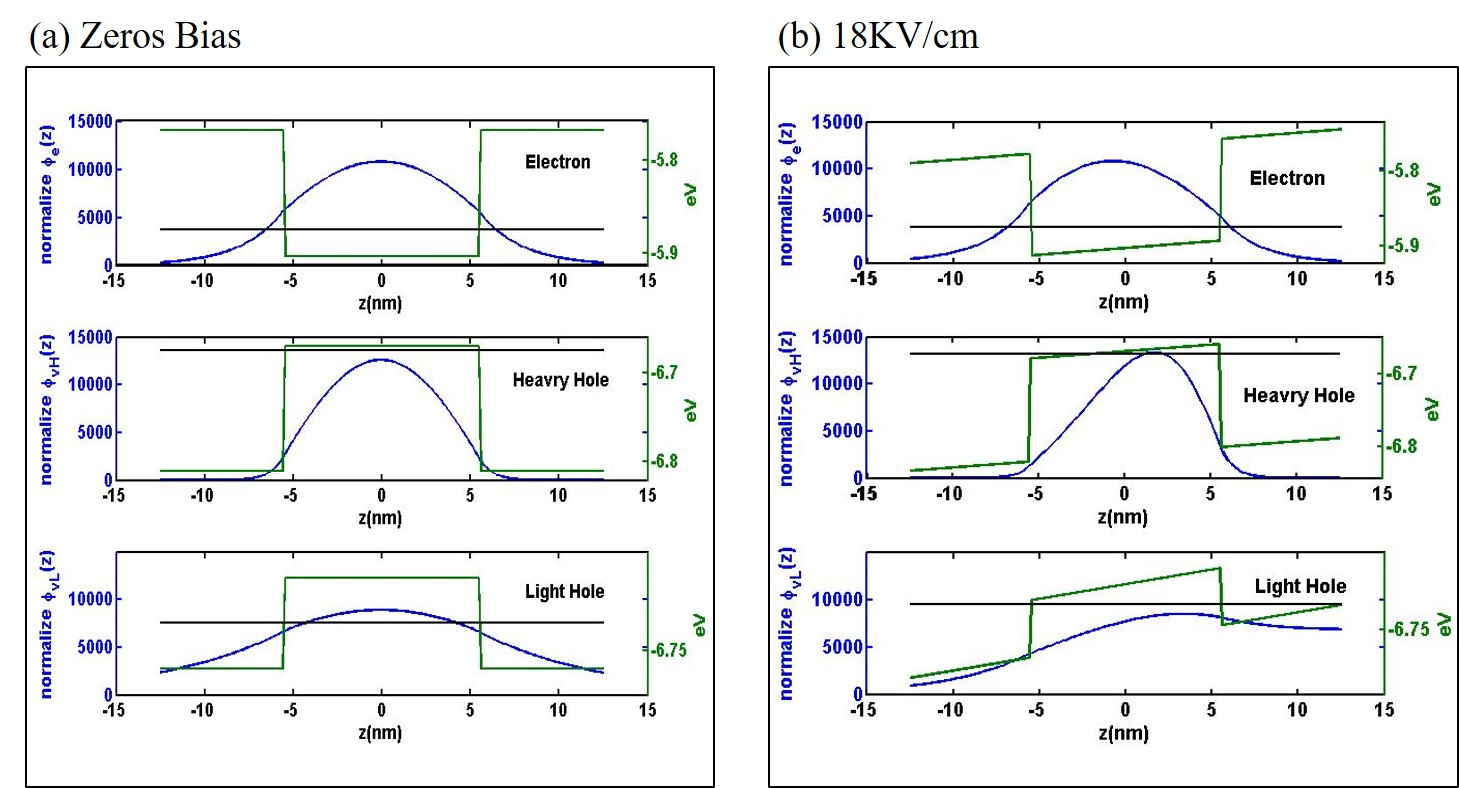
\includegraphics[width=14cm]{./Pictures/fig_ch2_bias_wavefunction.jpg}
	\caption{在不同偏压下电子,重空穴和轻空穴能带边沿,波函数,能级的变化,(a)无电场;(b)电场强度为2 KV/cm}
	\label{fig_ch2_bias_wavefunction}
\end{figure}

\subsection{优化设计}
\subsection{测试结果}
\section{波导尺寸的设计}
\subsection{光学性能的设计}
\subsection{电学性能的设计}
\section{本章小结}